\section{Various Types of Transmission Lines}\label{lec:lec15}
A final aspect of our discussion on transmission line is the characteristic impedance of common transmission lines in practice. At the beginning of our study, we saw various kinds of transmission line such as coaxial line, parallel wire, micro-strip structure etc., one would need to calculate the characteristics impedance of the line. Let us see the formulas used for calculating the characteristics impedance of the various transmission line. The most commonly used transmission line is the coaxial line commonly used for connection between electric equipments.

\subsection{Coaxial line}
The coaxial cable has an inner diameter $d$ outer diameter $D$ and dielectric constant $\epsilon_r$ for the medium separating the outer and inner conductor (see figure~\ref{fig:coaxialcable1}). Teflon is mostly used as the dielectric material to separate d from D and it has range of values from 2 to 4.
\begin{figure}[h]
\centering
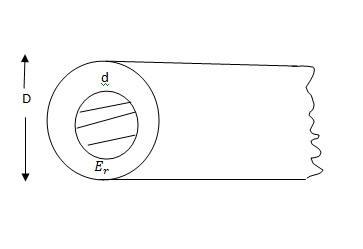
\includegraphics[width=1\linewidth]{./graphics/coaxialcable1}
\caption{coaxial line}
\label{fig:coaxialcable1}
\end{figure}
\begin{figure}[h]
\centering
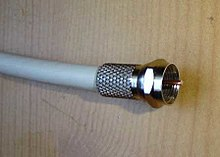
\includegraphics[scale=0.8]{./graphics/coaxialcable}
\caption{Typical image of a coaxial line}
\end{figure}

For this structure the characteristics impedance $Z_0$ is given by equation~\eqref{eqn:coaxialcable}.
\begin{equation}
Z_0 =\frac{138}{\sqrt{\epsilon_r}}\log(\dfrac{D}{d})
\label{eqn:coaxialcable}
\end{equation}
It shows that the characteristics impedance of a coaxial line depends on the ratio of outer to inner diameters, and the dielectric constant separating the inner and the outer diameters.

Let us take some typical values just to get a feel of what kind of parameters are required to realize certain characteristics impedance, say $\epsilon_r$=4, 
\begin{dmath*}
Z_0 =\dfrac{138}{\sqrt{4}}\log(\dfrac{D}{d})
= 69\log(\dfrac{D}{d})
\end{dmath*}
This implies that
\begin{dmath*}
\frac{D}{d}=10^{\left(\dfrac{Z_0 }{69}\right)}
\end{dmath*}
What we see from this relationship is that the ratio of $\frac{D}{d}$ increases very rapidly as the characteristic of impedance $Z_0 $ increases. Suppose that $Z_0 = 69\varOmega$ then, $\dfrac{D}{d}= 10$ or $D=10d$. Similarly, when $Z_0 = 138$
\begin{dmath*}
\dfrac{D}{d}=10^{\left(\dfrac{138}{69}\right)}=10^{2}=100
\end{dmath*}
Therefore $D=100d$.

Thus, the size of the outer conductor compared to the inner conductor increases very rapidly as the characteristics impedance of the line increases. This implies that the coaxial structure is more suited for realizing low characteristics impedances and that is the reason why typically the lines which are used as coaxial lines have characteristics impedance that lie around $50\varOmega$ to $75\varOmega$. If we say let us realize a characteristics impedance of 200 or 300 Ohms with the same structure, $\frac{D}{d} = 10^{\left(\dfrac{300}{69}\right)} = 22275.4$ which is obviously an outrageous value of $\frac{D}{d}$ and this size will be physically unreliable. Hence, the coaxial structure is intrinsically more suited for realizing low characteristics impedances of order $50\varOmega$ or $75\varOmega$. Typically the coaxial cables are standardized for $50\varOmega$, however when we go for antenna application we get a cable that has $75\varOmega$ characteristics impedance and the reason is that the antenna that is mostly used in practice that is, the \emph{half wave dipole}\index{half wave dipole} has input impedance very close to $75\varOmega$ as we shall see in later chapters. So just from the compatibility point of view of the impedances, whenever we use the coaxial cables for the antenna, we use the cable which is having a characteristics impedance of $75\varOmega$. However for most of other application of high frequency equipment the impedance has been almost standardized to $50\varOmega$.

\subsection{Parallel wire transmission line (balanced)} 
As the name suggest it has two conductors which are parallel with conductor diameter $d$ and separation between the two conductors as $D$ (see figure~\ref{fig:parallelwiretx}). Normally this arrangement is used in the air, so that the dielectric material separating these two conductors is air with $\epsilon_r=1$. However there are some applications where they are insulated from each with an insulating material and then encapsulated in a material casing; in this case, $\epsilon_r\neq1$. Such a structure is common in a overhead power line or a \emph{flat ribbon cable}\index{flat ribbon cable} used to connect a \emph{yagi antenna}\index{yagi antenna} to a television.
\begin{figure}[h]
\centering
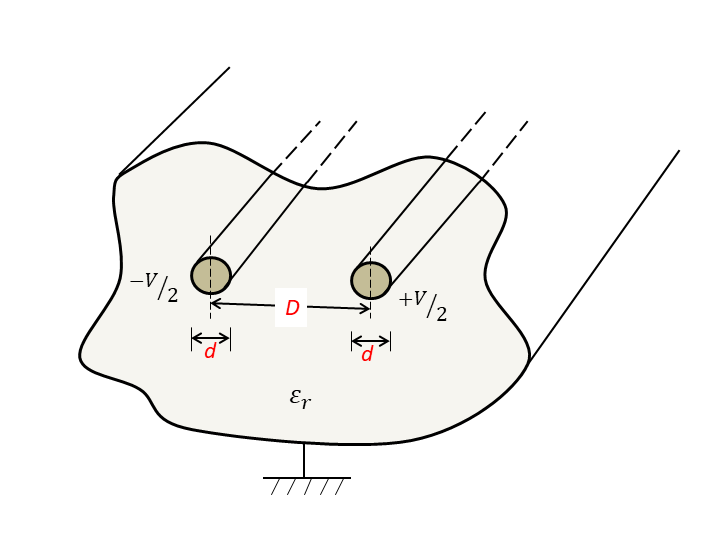
\includegraphics[width=1\linewidth]{./graphics/parallelWireTX}
\caption{Parallel Wire Transmission Line}
\label{fig:parallelwiretx}
\end{figure}

In the case where there is no air medium, we have a plastic encapsulation with $\epsilon_r\neq1$. The characteristics impedance of this structure is given by equation~\ref{eqn:parallelwiretx}.
\begin{equation}
Z_0 =\dfrac{276}{\sqrt{\epsilon_r}}\log(\dfrac{2D}{d})
\label{eqn:parallelwiretx}
\end{equation}

When air is the dielectric, $\epsilon_r$=1, so that
\begin{equation}
Z_0 = 276\log(\dfrac{2D}{d})
\label{eqn:parallelwiretxair}
\end{equation}
We can only make $D$ as small as possible to vary $Z_0 $. if $D\approx d$ that is, almost close to each other then 
\begin{dmath*}
Z_0 = 276\log(\dfrac{2d}{d})
=276\log(2)
=82.8\varOmega
\end{dmath*}
So minimum realizable value of $D$ is when $D = d$, and at that point $Z_\min=82.2\varOmega$. Suppose $\frac{D}{d}=5$, then
\begin{dmath*}
Z_0 =276\log(2\times5)
=276\log(10)
=276\varOmega
\end{dmath*}
As we can see for the parallel wire (balanced) structure, realizing low impedance is more difficult compared to coaxial cables. This is because we cannot realize impedance less than $82.8\varOmega$. However we can realize high impedance easily. Since we are talking about two conductor which are parallel, separating them to vary $D$ is very easy.

This kind of transmission line intrinsically is used for realizing high characteristics impedance. They are also used in telephone lines\textemdash\;all the telephone lines which are seen in towers are in the form of parallel wire lines. So generally, the parallel wire transmission line are used in that application where one would like to realize high impedances or conversely, when one would have to give such a structure a high impedance. So the coaxial structure and parallel wire structure are complimenting in terms of characteristics impedance. The coaxial cable structure can give low impedances easily and are difficult to get high impedances from. Whereas the parallel lines will easily give high impedance but are difficult to get low impedance from. Typically for a parallel wire transmission line the characteristics impedance is $Z_0 =300\varOmega$ or $Z_0 =600\varOmega$ so the parallel wire transmission line are also standardized to a fixed characteristics impedance.

\subsection{Microstrip line structure}\index{microstrip line}
The third structure in practice is the microstrip line structure and this structure is realized in practice at microwave frequencies for making circuits. Also, whenever we have a printed circuit board configuration the microstrip line is the kind of transmission line used (see figure~\ref{fig:microstrip}). The characteristics impedance of the structure depends on the dielectric $\epsilon_{r}$ and the ratio of $\frac{W}{h}$. The characteristic impedance for this structure is given as equation~\ref{eqn:microstrip}
\begin{figure}[h]
\centering
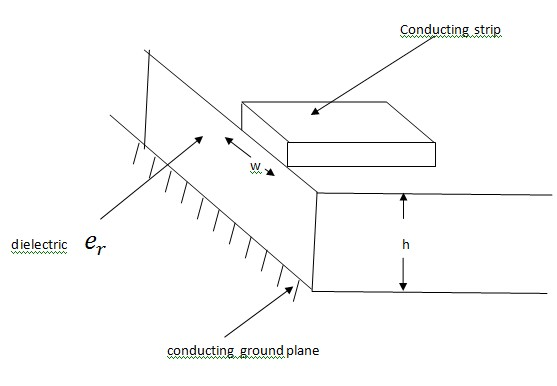
\includegraphics[width=1\linewidth]{./graphics/microstrip}
\caption{Microstrip line}
\label{fig:microstrip}
\end{figure}

\begin{equation}
Z_0 =\dfrac{377}{\left(\sqrt{\epsilon_r}\dfrac{W}{h}+2\right)}
\label{eqn:microstrip}
\end{equation}
At microwave frequencies, one can use a substrate like alumina as the dielectric which has a high value of dielectric constant (as high as 9.8). The dielectric constant value may have very wide range and $\frac{W}{h}$ can vary by a very wide range, so that we can realize a wide range of characteristic impedance. Using high $\epsilon_r$ we can realize low $Z_0$ and high $Z_0$ with small $\epsilon_r$.

We can vary the impedance by a large amount by changing $\frac{W}{h}$ ratio. Such that at high frequencies, we standardize the frequency to $50\varOmega$, if we are to connect it to a coaxial cable or make it have high impedance (maybe if we want to connect it to the parallel wire transmission line). There is a small difference however between these two connections and that is if we take a structure which is the coaxial cable structure with inner and outer conductor, we can connect voltage to the inner conductor and ground the outer conductor as shown in figure~\ref{fig:microstripvar}.
\begin{figure}[h]
\centering
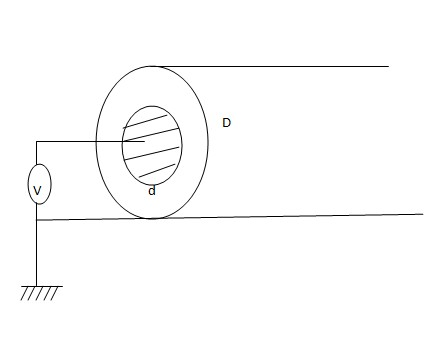
\includegraphics[width=1\linewidth]{./graphics/ground}
\caption{Variable Microstrip Line Structure}
\label{fig:microstripvar}
\end{figure}

It shows that a coaxial cable has a centre conductor which is connected to a voltage source and the outer conductor is grounded. This configuration is the same for the micro-strip line structure. We have the ground plane and the strip which carries voltage relative to the ground plane. So in both cases, above the ground is defined and the voltage is applied with respect to ground. However comparing this with the parallel wire structure, this is a completely floating structure and the ground is not defined for this structure. We can either say one of these conductors is at ground or zero potential while the other is at $V$ or we say that there is a virtual ground in between them somewhere at the middle with one cable at $\frac{+V}{2}$ and the other at $\frac{-V}{2}$. Hence this structure for which the ground is not defined is a floating structure while the other two have a well defined ground and the voltage is applied between the ground and the conductor.

The other two structures are called \emph{unbalanced structures}\index{unbalanced structure} and the parallel wire transmission line is called a \emph{balanced structure}\index{balanced structure}. Whenever we make connection between balanced and unbalanced lines,two things we see is that first impedance has to be matched at the junction, secondly since you are bringing now a connection between a balanced floating structure and an unbalanced structure,you require some transformer in between which can connect voltage from one bias structure to another bias structure. This device is called a \emph{balance to unbalanced transformer} or \emph{BALUN}\index{balun}.So a structure which matches the impedance as well as the nature of the cables is called BALUN\footnote{
An acronym from the words BALanced and UNbalanced
} as shown in figure~\ref{fig:balun}
\begin{figure}[h]
\centering
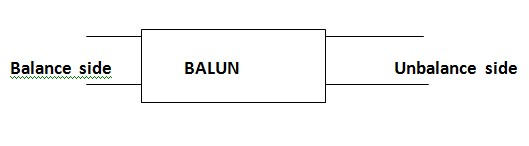
\includegraphics[width=1\linewidth]{./graphics/balun}
\caption{Boxview model of a BALUN}
\label{fig:balun}
\end{figure}
\begin{figure}[h]
\centering
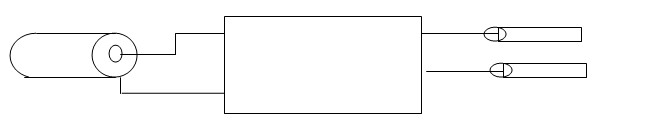
\includegraphics[width=1\linewidth]{./graphics/balun2}
\caption{Typical Application of a BALUN}
\label{fig:balun2}
\end{figure}

A typical application as shown in figure~\ref{fig:balun2} is when we make a connection between a \emph{yagi antenna}\index{yagi antenna} and a television. This is the most visible application you can see around, of course there are many other high frequency application of the \emph{BALUN}\index{balun}. Practically when using a \emph{yagi antenna} connected to a television, the signal from the antenna is sent using a \emph{flat ribbon cable}\index{flat ribbon cable} connected to the \emph{BALUN}\index{balun} structure which is a blackbox seen behind a television set. Typically, the connector at the back of a television set is a coaxial connector so it is unbalanced. The impedance of the coaxial connector is 50$\varOmega$, but for the \emph{flat ribbon cable}\index{flat ribbon cable} coming from the antenna, it is much different compared to 50$\varOmega$. So normally we introduce a small box which is the \emph{BALUN}\index{balun} and it transforms the impedance from the \emph{flat antenna ribbon cable} balanced structure to the unbalanced structure. If this is not done, there is the possibility that the reflection from the junctions will appear in form of ghosts on the television. So appropriate transformation of impedance on the line and also connecting balanced to unbalanced side of the network properly with the help of a \emph{BALUN}\index{balun} improves the quality of the reception with any high frequency signal. This essentially conclude our discussion on the transmission line.

\section{Conclusion}
Let us recap what we have done in this very important aspect of high frequency circuit called transmission line. We saw the limitation of the analysis of the lumped circuits that is as we go to high frequency,the size of the component becomes comparable to wavelength and then the voltage and current cannot be assumed constant along any electronic component, so we introduced the concept of the \emph{distributed element}. We studied the \emph{transit time}\index{transit time} effect and from there we derived the relationship between voltage and current for high frequency circuits that is, for circuits where the wavelength becomes comparable to the dimensions of the components\textemdash\;transit time effect cannot be neglected. We saw that the relationship were in the form of differential equations whose solution turned out to be that of a wave equation. So in general at high frequencies the voltage and current exist in the form of waves in the circuits.

Then we studied the superposition of these waves and we saw that in general we got a standing wave. We also investigated what conditions lead to two waves which are traveling in opposite directions or which lead to standing waves. So we introduced the concept of voltage \emph{reflection coefficient}\index{reflection coefficient}, which we discussed as the measure of energy reflected away from the load.

Then we introduced the concept of \emph{matching condition}\index{matching condition} which means that if a load impedance is equal to the characteristics impedance, the energy is transferred from the generator to the load efficiently and there is no reflection on the line. We then studied the impedance transformation characteristics of the transmission lines. Then we looked at many applications of transmission line which are \emph{as a circuit element}, \emph{as a resonant circuit}, \emph{as a voltage/current step up transformer} and \emph{as a matching transformer}.

Lastly, we looked at the characteristics impedance for various structures which are used as transmission line at high frequencies. For the coaxial cable, we concluded that its characteristics impedance is rather low and that it is difficult to realize high characteristics impedance using the coaxial structure. On the contrary the parallel wire structure is more capable of giving high characteristics impedances. We also looked at some applications where the parallel and coaxial transmission line could be used and the lastly, was the microstrip line structure which we studied to be normally seen at microwave frequencies of few GHz, its connection on a printed circuit board, and lastly using a \emph{BALUN}\index{balun} to connected balanced and unbalanced structures in other to prevent reflections.

Today computer speed reach GHz and transmission line effects is going to play a very prominent role in the circuit design. Few decades back when the frequencies where not very high, electronics circuit design was quite simple, all the transmission line effect where not playing a role in the circuit. However when circuit chips are operated at frequencies of few GHz (computers are soon operating at frequencies of a few GHz), the reflections, the mismatching and so on which we discussed become very vital in designing the electronic circuits. So in today's electronic circuits, the concept of transmission line plays a very important role. The subject of transmission line has become very important for recent years because of these high speed electronic circuits which are now part of our everyday life.

\section{Exercises}
\begin{ExerciseList}
\Exercise[label={ex151}]
Find the characteristic impedance each of the following transmission lines:
\begin{enumerate}[(a)]
\item a coaxial cable using a solid polyethylene dielectric having $\epsilon_r = 2.3$ with inner radius 0.5mm and outer radius 1.5mm; 
\item a parallel wire line with wire radius 0.5mm and spacing 1mm; 
\item a microstrip line with substrate thickness 1mm, dielectric constant 4.5, and strip width 1mm.
\end{enumerate}
\Answer[ref={ex151}]
Solution to exercise~\ref{ex151}.
\Exercise[label={ex152}]
A 600-$\varOmega$ transmission line is 150m long, operates at 400kHz with $\alpha = 2.4\times 10^{-3}$ Np/m and $\beta = 0.0212$ rad/m, and supplies a load impedance $Z_L = 424.3\angle45^{\circ}\varOmega$. Find the length of line in wavelengths, $\Gamma_L, \Gamma(L)$, and $Z(L)$. For a received voltage $V(0) = 50\angle0^{\circ}$V, find $V(L)$, the position on the line where the voltage is maximum, and the value of $|V|_\max$.
\Answer[ref={ex152}]
(a) $\Gamma_L = 0.45\angle116.6^{\circ}$, $\Gamma(L) = 0.22\angle113.6^{\circ}$, $Z(L) = 502.7\angle22.8^{\circ}\varOmega$; (b) $V(L) = 75.0\angle167.3^{\circ}$V, $|V|_\max = 85.5$V at $x = 0.162\lambda$.
\Exercise[label={ex153}]
A 70-$\varOmega$ high frequency lossless line is used at a frequency where $\lambda = 80cm$ with a load at $x = 0$ of $(140 + j91)\varOmega$. Use the Smith chart to find the following:
\begin{enumerate}[(a)]
\item The reflection coefficient $\Gamma_L$ 
\item VSWR
\item The distance to the first voltage maximum from the load
\item The distance to the first voltage minimum from the load
\item The impedance at the first voltage maximum
\item The impedance at the first voltage minimum
\item The input impedance for a section of line of length that is $54cm$ long, and
\item The input admittance for a section of line of length that is $54cm$ long.
\end{enumerate}
\Answer[ref={ex153}]
Solution to exercise~\ref{ex152}.
\end{ExerciseList}